\chapter{Descrizione delle sorgenti sviluppate}

\section{Dal primo al terzo prototipo}

\section{Attuale schema operativo}
\subsection{Alimentatore e trigger ottico}
\subsection{Testa}

\section{Funzionamento e applicazione}
\subsection{Segnale elettrico}

\paragraph{Tensione}Vengono effettuate misure della tensione in uscita dal secondario utilizzando una sonda per l'alta tensione, al variare dei parametri del segnale in ingresso: frequenza ($f$) e duty cycle ($\Delta t$). Scelta la frequenza di lavoro, viene variata la duty cycle in un range utile, considerando il tempo necessario al terminare delle oscillazioni del segnale prima dell'arrivo di una nuova onda quadra (per frequenze maggiori si potrà arrivare a duty cycle minori).
Le misure vengono rilevate con un oscilloscopio in grado di salvare tutta la forma dell'onda misurata. Si ottengono curve come in figura \ref{fig:tensione_es}. La risoluzione della misura (V/div) viene variata in modo da avere l'errore di misura minore possibile.
Le prime misure effettuate sono una verifica della tensione in uscita dal circuito secondario in aria, senza aggiunta di gas.
Per le misure successive viene immesso nella sezione finale della sorgente del gas He, con un flusso di $\SI{2}{\litre/\minute}$.

\begin{figure}
\centering
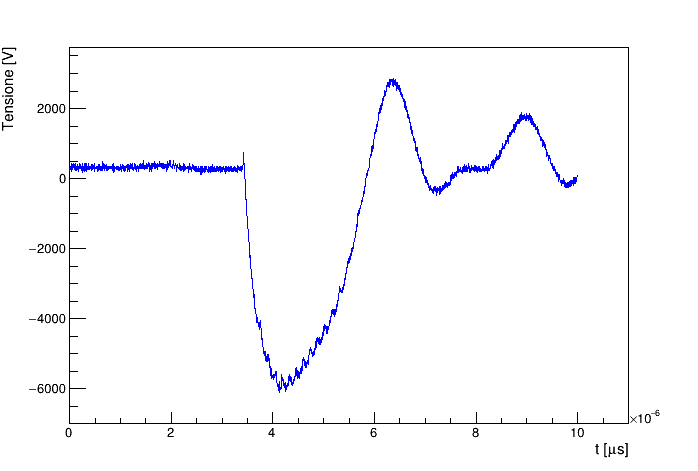
\includegraphics[width=.7\textwidth]{Immagini/tensione_es_2.png}
\caption{Esempio di misura di tensione, $f = \SI{5}{\kilo\hertz}$ e $\Delta t = \SI{16}{\micro\second}$}
\label{fig:tensione_es}
\end{figure}

\paragraph{Corrente}Vengono effettuate misure della corrente passante tra la sorgente di plasma e un bersaglio metallico. Viene posta una piastra di rame (dimensioni $\SI{2}{\centi\metre} \times \SI{2}{\centi\metre} \times \SI{0.5}{\centi\metre}$) ad una distanza di $\SI{1}{\centi\metre}$ dall'elettrodo della sorgente. La piastra bersaglio viene collegata ad una sonda per la misura di corrente, per la quale un segnale letto dall'oscilloscopio come $\SI{10}{\milli\volt}$ corrisponde a $\SI{10}{\milli\ampere}$.
Viene inoltre collegata all'uscita del circuito secondario la sonda per l'alta tensione usata precedentemente, in modo da visualizzare contemporaneamete la tensione e la corrente in uscita dalla sorgente. Nuovamente vengono effettuate misure al variare dei parametri del segnale in ingresso: frequenza ($f$) e duty cycle ($\Delta t$), con le stesse modalità delle misure di tensione.
Tutte le misure sono effettuate con flusso di gas He pari a $\SI{2}{\litre/\minute}$.
Si ottengono curve come in figura \ref{fig:corrente_es}. Il picco di tensione è identico a quello misurato precedentemente, con valori tipici tra i $\num{3}$ e i $\SI{6}{\kilo\volt}$, coerenti con le scorse misure per il range di parametri utilizzato. La corrente presenta sempre un primo picco negativo ed un picco secondario positivo, con valori tra i $\num{2}$ e i $\SI{12}{\milli\ampere}$.

\begin{figure}
\centering
\subfloat[][Tensione]
  {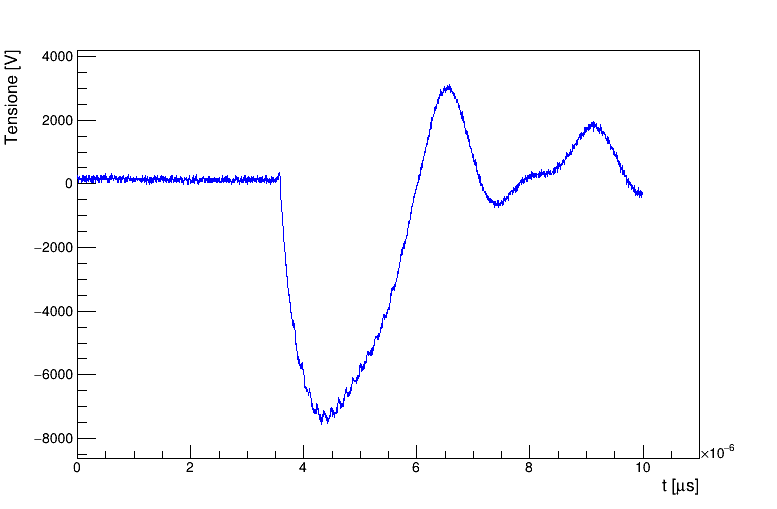
\includegraphics[width=.48\textwidth]{Immagini/tensione_es.png}}
\subfloat[][Corrente]
  {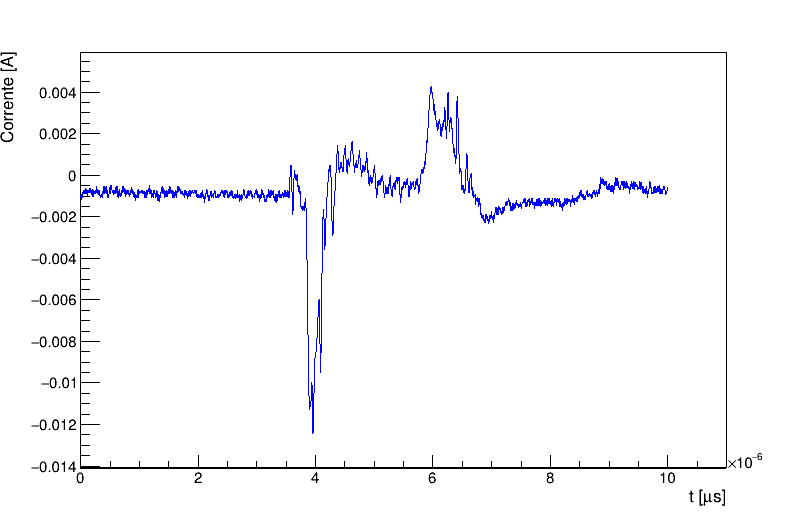
\includegraphics[width=.48\textwidth]{Immagini/corrente_es.png}}
\caption{Esempio di misure di corrente e tensione per $f = \SI{5}{\kilo\hertz}$ e $\Delta t = \SI{24}{\micro\second}$.}
\label{fig:corrente_es}
\end{figure}

\subsection{Forma e temperatura della \emph{plume} di plasma}


\subsection{Produzione specie gassose reattive}
Per caratterizzare il gas in uscita dalla sorgente vengono eseguite delle misure spettrometriche.

\paragraph{Righe spettrali}Lo scopo è di osservare in particolar modo le specie reattive dell'ossigeno e dell'azoto prodotte dalla sorgente, quindi vengono effettuate acquisizioni in tutto il range di lunghezze d'onda interessato (\SI{300}-\SI{900}{\nano\meter}) e centrate sulle righe relative alle molecole \ce{OH} (\SI{305.00}-\SI{313.00}{\nano\meter}), \ce{N_{2}} (\SI{668.00}-\SI{676.00}{\nano\meter}) e \ce{NO} (\SI{220.0}-\SI{290.0}{\nano\meter}). 

\paragraph{Composizione del gas}Si vuole osservare l'intensità relativa delle righe al variare del gas in ingresso, quindi la sorgente viene azionata con diverse miscele di gas. La misura standard viene effettuata con flusso di \ce{He}, nella solita modalità di funzionamento della sorgente. Vengono poi predisposte due ulteriori modalità di misura dove il gas viene fatto gorgogliare in una soluzione di acqua o di ammoniaca prima dell'inserimento all'uscita della sorgente, per arricchire i prodotti delle reazioni rispettivamente ioni \ce{OH} e di specie reattive dell'azoto.

\paragraph{Temperatura molecole} A partire dalla forma delle righe di alcune specie molecolari, è possibile stimare la temperatura alla quale avviene l'emissione misurata. Le emissioni dovute alla molecola \ce{OH} sono diverse righe compresi tra \SI{306}{\nano\meter} e \SI{310}{\nano\meter} (vedi articolo), dalle intensità variabili a seconda della temeperatura delle molecole. Le emissioni dovute a transizioni di stati rotazionali della molecola \ce{N_2} sono invece righe comprese tra \SI{326}{\nano\meter} e \SI{338}{\nano\meter} (vedi articolo). Entrambe le misure sono una stima della temperatura degli ioni che compongono il gas, ad esempio per l'\ce{OH} si avrà uno spettro del tipo presentato in Equazione \ref{eq:fitOH} (vedi articolo):
\begin{equation}
\begin{split}
&I_i (T) = I_{0,i} \exp{-\frac{E_n (T-T_0)}{T_0 T}} \\
&S_i(\lambda,T) = \frac{I_i(T)}{\sigma \sqrt{2\pi}} \exp{\frac{(\lambda - \lambda_i)^2}{2\sigma^2}}\\
&S(\lambda,T) = \sum_i S_i(\lambda,T)
\end{split}
\label{eq:fitOH}
\end{equation}

dove $I_i$ è l'intensità ad una determinata energia $E_n$ e $I_{0,i}$ è l'intensità misurata alla temperatura conosciuta $T_0$, mentre $S_i$ è la convoluzione di $I_i$ con una distribuzione gaussiana nelle $\lambda$ e lo spettro finale sarà la somma di tutti i picchi.

\subsection{Applicazione a campioni biologici}


\label{ch:sorgentemisure}
